\documentclass{aip-cp}

\usepackage[numbers]{natbib}
\usepackage{rotating}
\usepackage{graphicx}

\usepackage{bm}

% Document starts
\begin{document}

% Title portion
\title{Solution of the Neutronics Code Dynamic Benchmark by Finite Element Method}

\author[aff1]{A.V. Avvakumov}
\author[aff2]{P.N. Vabishchevich}
\author[aff3]{A.O. Vasilev\corref{cor1}}
\author[aff2]{V.F. Strizhov}
%\eaddress{anotherauthor@thisaddress.yyy}

\affil[aff1]{National Research Center "Kurchatov Institute", Moscow, Russia}
\affil[aff2]{Nuclear Safety Institute, Moscow, Russia}
\affil[aff3]{North-Eastern Federal University, Yakutsk, Russia}
\corresp[cor1]{Corresponding author: haska87@gmail.com}

\maketitle

\begin{abstract}
The objective is to analyze the dynamic benchmark developed by Atomic Energy Research for the verification of best-estimate neutronics codes. The benchmark scenario includes asymmetrical ejection of a control rod in a water-type hexagonal reactor at hot zero power. A simple Doppler feedback mechanism assuming adiabatic fuel temperature heating is proposed. The finite element method on triangular calculation grids is used to solve the three-dimensional neutron kinetics problem. The software has been developed using the engineering and scientific calculation library FEniCS. The matrix spectral problem is solved using a scalable and flexible toolkit SLEPc. The solution accuracy of the dynamic benchmark is analyzed by condensing calculation grid and varying degree of finite elements.
\end{abstract}

% Head 1
\section{INTRODUCTION}
The physical processes in a nuclear reactor \cite{duderstadt1976nuclear}
depend on distribution of neutron flux, whose mathematical description is based on the neutron transport equation \cite{stacey}. 
The general view of this equation is integro-differential one, and the required distribution of neutrons flux depends on time, energy, spatial and angular variables. As a rule, the simplified forms of the neutron transport equation are used for practical calculations of nuclear reactors. The equation system that is known as a multigroup diffusion approach is mostly used for reactor analysis \cite{marchuk1986numerical}
and is applied in most engineering calculation codes.

To increase calculational accuracy, nodal methods are widely used. These methods allow modelling on a rather coarse mesh.
The basic idea of a nodal method is to represent neutron flux within a calculational cell as a few-degree polynomial function or as a set of 1-D or 2-D functions. Nodal methods can be connected, in some respect, to the special variants of finite-element approximation \cite{grossman2007nodal}. We can note that it is more appropriate to use the standard procedures of increasing accuracy of the finite-element approximation for boundary problem solution with mesh refinement and using high-order finite elements.

The standard methods of approximate solutions of non-stationary problems are used for modelling of the dynamics of neutron-physical processes. The most attention is paid to two-level schemes with weights ($\theta$-method) \cite{Ascher2008},
the Runge-Kutta and Rosenbrock schemes \cite{Butcher2008} are used.
Let's note a special class of methods for modelling of non-stationary neutron transport in diffusion multigroup approximation, which is connected with multiplicative representation of solution --- space-time factorization methods and the quasistatic method \cite{chou1990three}.
The approximate solution is searched in the form of the product of two functions, one of which depends on time and is related to the amplitude, the second one (the shape function) describes the spatial distribution. It is difficult to check the accuracy of the approximate solution in such approach, in particular, while calculating the dynamic modes with complicated changes in neutron flux distribution.

The processes occurring in a nuclear reactor are essentially non-stationary. The stationary state of neutron flux, which is related to the critical state of the reactor, is characterised by local balancing of neutron absorption and and generation. This boundary state is usually described by solution of a spectral problem (Lambda Modes problem, $\lambda$-eigenvalue problem) provided that the fundamental eigenvalue (maximum eigenvalue) that is called $k$-effective of the reactor core, is equal to unity. In this case, the stationary neutron field is related with the corresponding eigenfunction. Calculations of $k$-effective of the reactor on the basis of the spectral Lambda Modes problem solution are obligatory for developing a new design of reactor installation.

%Time behaviour of nuclear reactor is deemed sometimes to be related to the deviation of $k$-effective from unity that involves, in particular, concept of reactivity. This is not justified, since, while calculating this parameter, the evolutionary nature of neutron redistribution processes (nonstationary systems of the equations) is considered in no way. The $k$-effective parameter deviates from unity, though quite weakly, but anyway such a solution, generally speaking, cannot be connected with the stationary solution of the problem. There is simply no such a solution. Thus, the attempts to correct the basic mathematical model of non-stationary neutron diffusion by introducing some correcting multipliers to achieve the strict criticality are not successful.

%The spectral parameter $\alpha$, which is not directly connected with $k$-effective, is proposed to be used instead of $k$-effective for more adequate characteristic of the dynamic nature of reactor. It is defined as the fundamental eigenvalue of the spectral problem (time-eigenvalue, $\alpha$-eigenvalue problem), which is connected with the non-stationary equations of neutron diffusion \cite{Bell1970,modak2007scheme,verdu20103d}.
%By analogy with the usual problems of heat conductivity (see, for example, \cite{luikov2012analytical,samarskii1996computational}) we consider the regular reactor mode. At large times the behavior of a neutron flux is asymptotic, and one can talk about space-time factorization solution, whose amplitude is $\exp(\alpha t)$, the shape function is the eigenfunction of the spectral problem. 
%
%Study of the dynamic processes can be based on the discrimination of symmetric and skew-symmetrical parts of the neutron transport operator. In this case, we can easily get the a priori assessments of stability in the corresponding norm, while assessing the operator of the symmetric part from below, and perform the analysis of used time approximations \cite{Samarskiibook,SamarskiiMatusVabischevich2002}. 
%To get this, the partial spectral problem is solved to find the fundamental eigenvalue $\delta$ of the Delta Modes spectral problem.


\section{PROBLEM STATEMENT}
Nonstationary process in nuclear reactor is modelled using multi-group diffusion approximation. Neutron flux dynamics is considered within two-dimensional or three-dimensional domain $\Omega$ ($\bm x = \{x_1, ..., x_d\} \in \Omega, \ d = 2,3$) with a convex boundary $\partial \Omega$. Neutron transport described by the system of equations:
\begin{equation}\label{1}
\frac{1}{v_g} \frac{\partial \phi_g}{\partial t} - \nabla \cdot D_g \nabla \phi_g + \Sigma_{rg} \phi_g - \sum_{g\neq g'=1}^{G} \Sigma_{s,g'\rightarrow g} \phi_{g'} = (1-\beta) \chi_g \sum_{g'=1}^{G} \nu \Sigma_{fg'} \phi_{g'} + \widetilde{\chi}_g \sum_{m=1}^{M} \lambda_m c_m , \quad 
 g = 1,2, ..., G .
\end{equation}
Here $\phi_g(\bm x,t)$ is the neutron flux in group $g$ at point $\bm x$ at time moment $t$,
$G$ is the number of energy groups,
$v_g$ is the effective neutron velocity of group $g$,
$D_g(\bm x)$ is the diffusion coefficient, 
$\Sigma_{rg}(\bm x,t)$ is the removal cross-section,
$\Sigma_{s,g'\rightarrow g}(\bm x,t)$ is the cross-section for scattering a neutron from group $g'$ to group $g$,
$\chi_g$ and $\widetilde\chi_g$ is the fraction of the of the fission neutrons and delayed neutrons in group $g$, 
$\nu\Sigma_{fg}(\bm x,t)$ is the generation cross-section in group $g$, 
$c_m$ is delayed neutron source density of $m$ type,  $\lambda_m$ is decay constant of the delayed neutron sources,
$M$ is the number of types of delayed neutrons.
The density of the delayed neutron sources is described by the equations:
\begin{equation}\label{2}
 \frac{\partial c_m}{\partial t} + \lambda_m c_m = \beta_m \sum_{g=1}^{G} \nu \Sigma_{fg} \phi_g,
 \quad m = 1,2, ..., M, 
\end{equation} 
where $\beta_m$ --- fraction of delayed neutrons of $m$ type and:
\[
 \beta = \sum_{m=1}^{M} \beta_m .
\] 
The albedo-type conditions are set at the boundary $\partial \Omega$:
\begin{equation}\label{3}
 D_g\frac{\partial \phi_g}{\partial n} + \gamma_g \phi_g = 0, \quad 
 \quad g = 1,2, ..., G ,
\end{equation}
where $n$ is the outer normal vector to the boundary $\partial \Omega$.

We considered a boundary problem for the system of equations (\ref{1}), 
(\ref{2}) with boundary conditions (\ref{3}), and the initial conditions:
\begin{equation}\label{4}
 \phi_g(\bm x,0) = \phi_g^0(\bm x), 
  \quad  g = 1,2, ..., G ,
 \quad   c_m(\bm x,0) = c_m^0(\bm x), 
  \quad  m = 1,2, ..., M .
\end{equation} 

Let's write the boundary problem (\ref{1})-(\ref{4}) in operator form. The vector $\bm \phi = \{\phi_1, \phi_2, ..., \phi_G\}$, $\bm c^0 = \{ c_1^0,  c_2^0, ...,  c_M^0 \}$ and matrices are defined as follows:
\[
 V = (v_{g g'}),
 \quad v_{g g'} = \delta_{g g'} v_g^{-1},
\] 
\[
 D = (d_{g g'}),
 \quad d_{g g'} = - \delta_{g g'} \nabla \cdot D_g \nabla,
\] 
\[
 S = (s_{g g'}),
 \quad  s_{g g'} =  \delta_{g g'} \Sigma_{rg} - \Sigma_{s,g'\rightarrow g} ,
\] 
\[
 R = (r_{g g'}),
 \quad  r_{g g'} = (1-\beta)\chi_g \nu \Sigma_{fg'}, \\
\]
\[
 B = (b_{g m}),
 \quad b_{g m} = \widetilde{\chi}_g \lambda_m, \\
\] 
\[ 
 \Lambda = (\lambda_{m m'}),
 \quad  \lambda_{m m'} = \lambda_m \delta_{m m'}, \\
\]
\[ 
 Q = (q_{mg}),
 \quad  q_{mg} = \beta_m \nu \Sigma_{fg},
\]
\[
L = (l_{g g'}), \quad l_{g g'} = \delta_{g g'} \gamma_g,
\]
\[
g, g' = 1,2, ..., G,
\] 
where $\delta$ is the Kronecker symbol.

We shall use the set of vectors $\bm \phi$, whose components satisfy the boundary conditions (\ref{3}). Using the set definitions, the system of equations can be written in the form of first-order equation of evolution:
\begin{equation}\label{5}
V \frac{d \bm \phi}{d t} + (D+S) \bm \phi = R \bm \phi + B\bm c,
\quad
\frac{d \bm c}{d t} + \Lambda \bm c = Q \bm \phi. 
\end{equation}  

The Cauchy problem is solved for (\ref{5}), when
\begin{equation}\label{6}
D\frac{d \bm\phi}{d n} + L \bm \phi = 0, 
\quad \bm \phi(0) = \bm \phi^0,
\quad  \bm c(0) = \bm c^0,
\end{equation} 
where (see (\ref{4})) $\bm \phi^0 = \{ \phi_1^0,  \phi_2^0, ...,  \phi_G^0 \}$, $\bm c^0 = \{ c_1^0,  c_2^0, ...,  c_M^0 \}$.

To characterize the reactor dynamic processes described by Cauchy problem 
(\ref{5}), (\ref{6}), let's consider a spectral 
problem \cite{Bell1970,stacey}. The following spectral problem is usually solved:

\begin{equation}\label{7}
 (D+S) \bm \varphi = \lambda^{(k)} \left ( R \bm \varphi  +  B \bm s \right ), 
 \quad
 \Lambda \bm s = \lambda^{(k)} Q \bm \varphi .
\end{equation}
This problem (\ref{7}) is known as the Lambda modes problem for a given configuration of the reactor core.
The minimal eigenvalue is used for characterisation of neutron field, thus 
\[
 k = \frac{1}{\lambda^{(k)}_1}  
\] 
is the effective multiplication factor ($k$-effective).
The value $k = 1 / \lambda^{(k)}_1 = 1$ is related to the critical state of the reactor, and the corresponding eigenfunction $\varphi_1(\bm x)$ is the stationary solution of the equation (\ref{7}).
At $k > 1$, one can speak about supercriticality, at $k < 1$  --- about subcriticality.

%\begin{eqnarray}
%p_{t_{10,1}}&=&\left(\frac{N_{cu}^2}{ N_c ^2}\right)\left(\frac{N_{ar}^2}{N_a^2}\right)\left(\frac{N_{ar}-1}{N_{ar}}\right),\\
%p_{t_{10,2}}&=&\left(\frac{N_{cu}^2}{ N_c ^2}\right)\left(\frac{N_{ar}}{N_a^2}\right).
%\end{eqnarray}

\section{DISCRETIZATION}
Define uniform grid
$\omega = \{ t^n=n \tau, \quad n = 0,1,...,N, \quad \tau N = T \}$ and use next notations $\bm\phi^n = \bm\phi(\bm{x}, t^n)$, $\bm c^n = \bm c(\bm{x}, t^n)$.

For delayed neutron source equation we use numerical-analytical method for the construction of approximations in time.
The equation (\ref{2}) in the equivalent form:
\[
  \frac{\partial e^{\lambda_m t}  c_m}{\partial t} = \beta_m  e^{\lambda_m t} \sum_{g=1}^{G} \nu \Sigma_{fg} \phi_g,
 \quad m = 1,2, ..., M .
\] 
After integration on time interval [$t^{n}$, $t^{n+1}$] one can obtained:
\begin{equation}\label{8}
c_m^{n+1} = e^{-\lambda_m\tau} c_m^n + \beta_m \int_{t_n}^{t_{n+1}}e^{\lambda_m (t-t^{n+1})} \sum_{g=1}^{G} \nu \Sigma_{fg} \phi_g d t,
 \quad m = 1,2, ..., M.
\end{equation}

When using a fully implicit scheme we take the integrand on the right side at $t = t^{n+1}$. For the system of equations (\ref{5}) fully implicit scheme can be written as:
\begin{eqnarray*}
V \frac{\bm\phi^{n+1}-\bm\phi^n}{\tau}+(D+S) 
\bm \phi^{n+1} = R \bm \phi^{n+1} + B\bm c^{n+1},
\quad
\bm{c}^{n+1} = \widetilde{\Lambda}\bm{c}^{n} + \tau Q \bm{\phi}^{n+1},
\end{eqnarray*}
where
\[
\widetilde{\Lambda} = (\widetilde{\lambda}_{mm'}), \quad \widetilde{\lambda}_{mm'} = \delta_{mm'} e^{-\lambda_m\tau},
 \quad m, m' = 1,2, ....,M .
\]

For spatial approximation we use the finite element method\cite{quarteroni}.
Let $H^1(\Omega)$ -- Sobolev space, $v \in H^1$: $v^2$ and $\vert\nabla v\vert^2$ have a finite integral in $\Omega$. For $\bm v = \{v_1, v_2, ..., v_d\}$ define $V^d = [H^1(\Omega)]^d$. For test functions use notations $\bm \xi  = \{\xi_1, \xi_2, ..., \xi_G\}$, $\bm \zeta  = \{\zeta_1, \zeta_2, ..., \zeta_M\}$.\\
In variation formulation we are looking for $\bm \phi \in V^D, \ \bm c \in V^M$ such that:
\begin{eqnarray*}
\int_\Omega \left (V \frac{\bm\phi^{n+1}-\bm\phi^n}{\tau} + S
\bm \phi^{n+1} \right )\bm \xi  d\bm x 
+ \int_{\Omega} \sum_{g=1}^{G} D_G \nabla \phi^{n+1}_g \nabla  \xi_g d\bm x + \\
+ \int_{\partial \Omega} \sum_{g=1}^{G} \gamma_g \phi^{n+1}_g \xi_g d\bm x
= \int_\Omega R \bm \phi^{n+1}\bm \xi d\bm x + \int_\Omega B\bm c^{n+1}\bm \xi d\bm x,
\\
\int_\Omega \bm{c}^{n+1}\bm \zeta d\bm x = \int_\Omega \widetilde{\Lambda}\bm{c}^{n}\bm \zeta  d\bm x + \int_\Omega \tau Q \bm{\phi}^{n+1}\bm \zeta  d\bm x
\end{eqnarray*}
for all $\bm \xi  \in V^D, \ \bm \zeta  \in V^M$.
\\
Next, introduce a discrete function spaces $V_h^D \subset V^D$, $V_h^M \subset V^M$ and define discrete variational problem. The standard Lagrangian finite elements of degree p =
1, 2 are used \cite{brenner}. The software has been developed using the engineering and scientific calculation library FEniCS \cite{fenics}. The SLEPc package has been used for numerical solution of the spectral problems.

\section{AER-2 BENCHMARK}
A three-dimensional hexagonal dynamic benchmark \cite{grundman} models a peripheral control rod ejection in a VVER-440 core with neutron kinetics and simple adiabatic Doppler feedback. The transient to be analyzed is a short superprompt critical power excursion terminated by the Doppler feedback without any reactor scram.  The power of the reactor is limited by the continuous accumulation of heat in the fuel.
\begin{figure}[!h]
  \centerline{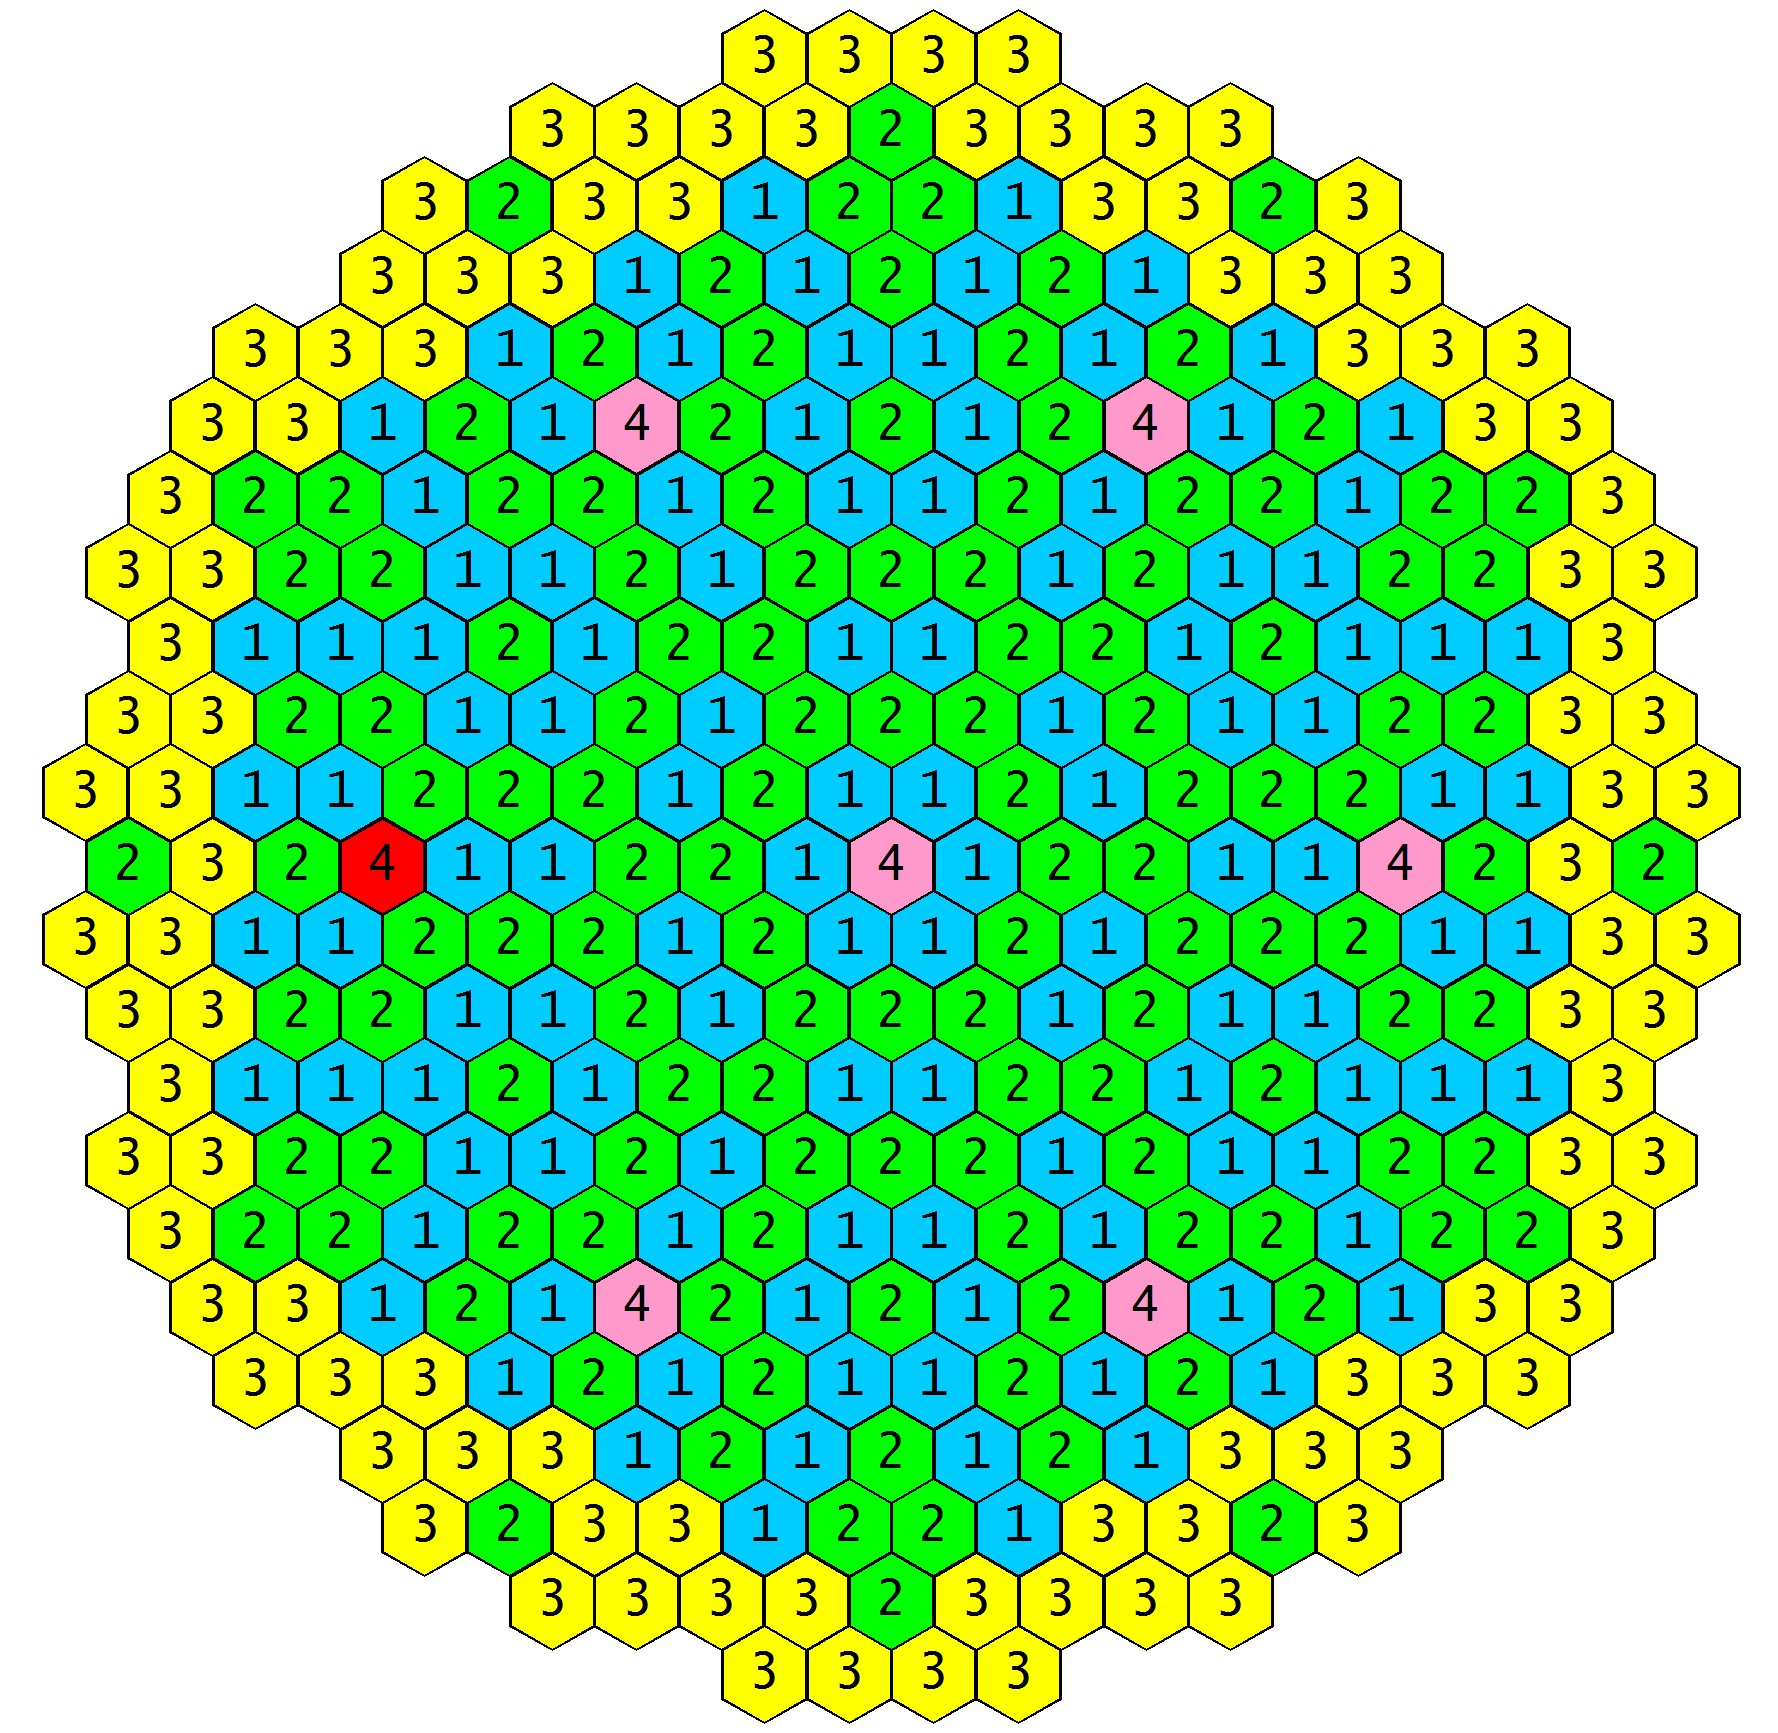
\includegraphics[width=200pt]{geo_cartogramm.jpg}}
  \caption{Load map of fuel assemblies.}
  \label{fig:1}
\end{figure}
\begin{figure}[!h]
  \centerline{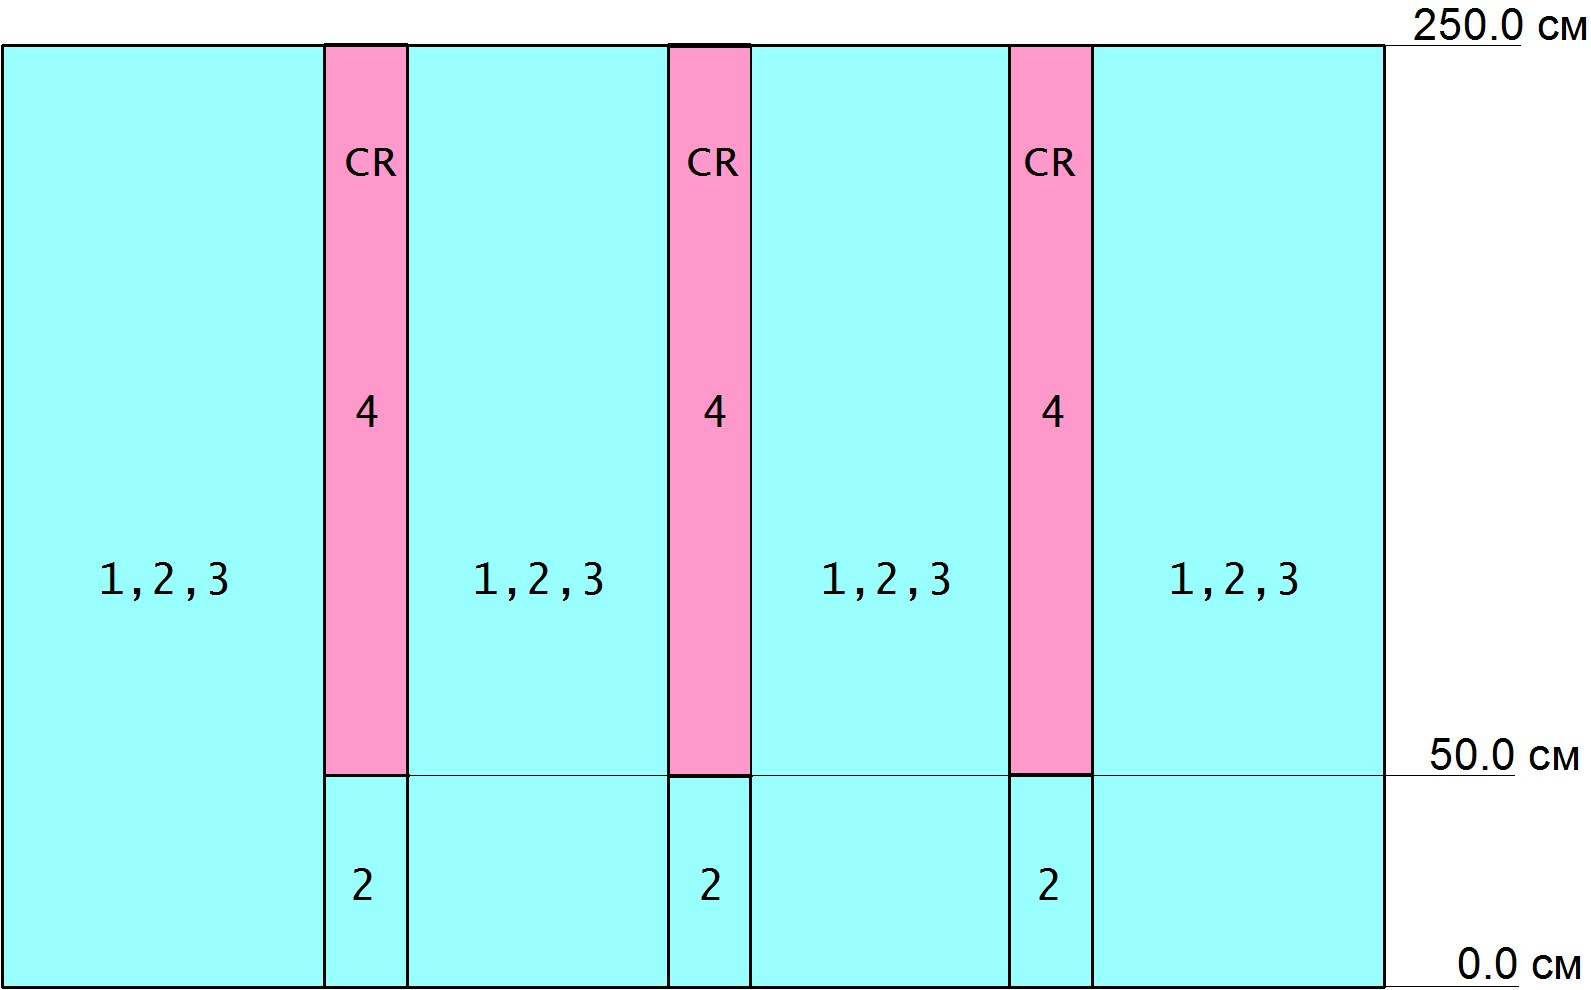
\includegraphics[width=200pt]{geo_axial.jpg}}
  \caption{Axial cross-section of the core.}
  \label{fig:2}
\end{figure}

The initial configuration of the considered VVER-440 reactor is close to the standard configuration with fresh fuel. Core height is 250 cm, fuel assembly pitch equals 14.7 cm. The position of the lower end of the absorber of the control rod is 50 cm from the bottom of core. Fig. \ref{fig:1} the load map of fuel assemblies of three types, among them first three types are fuel assemblies and the fourth type describes control assemblies.  The control assemblies consist of absorber type 4 in the upper part and fuel of type 2 in the lower part. The position of the ejected rod is marked as a red hexagon. The axial cross-section of the core with initial position of the control rods is given in Fig. \ref{fig:2}. Axial and radial reflector is described by given boundary conditions. 

Diffusion neutronics constants in the common notations are given in Table \ref{t-1}. The boundary
conditions at the core boundary describing the properties of radial and axial reflectors are contained in table \ref{t-2}. The number of delayed neutron groups $M = 6$. There is only one set of constants for all nodes. The constants of delayed neutrons are given in Table \ref{t-3}. The total fraction of delayed neutrons is reduced to $\beta = 0.005$ which increases the reactivity to $\beta$ and stands also for the higher content of Plutonium . The reactivity worth of the absorbers was increased by change of cross sections. It leads to a reactivity insertion of about $2\beta$ by the rod ejection. It was chosen to cover any considered transient of this type in the existing plants. The problem is solved at $v_1 = 1.25 \cdot 10^7 $cm/s и  $v_2 = 2.5 \cdot 10^5$cm/s.
\begin{table}[!h]
\caption{Diffusion neutronics constants for AER2 benchmark.}
\label{t-1}
\tabcolsep7pt\begin{tabular}{cccccccc}
\hline
Mat & $D_1$(cm)  & $D_2$(cm)  & $\Sigma_{r1}$(cm$^{-1}$) & $\Sigma_{r2}$(cm$^{-1}$) & $\Sigma_{s,1\to 2}$(cm$^{-1}$) &  $\nu\Sigma_{f1}$(cm$^{-1}$) & $\nu\Sigma_{f2}$(cm$^{-1}$) \\
\hline
1&1.3466 & 0.37169 & 0.008362 & 0.064277 & 0.016893 & 0.0044681 & 0.07407 \\
2&1.3377&0.36918&0.008797&0.079361&0.015912&0.0055576&0.10626 \\
3&1.3322&0.36502&0.00947&0.1001&0.014888&0.0070693&0.15029\\
4&1.1953&0.19313&0.2&0.8&0.022264&0.0&0.0\\
\hline
\end{tabular}
\end{table}

\begin{table}[!h]
\caption{Boundary conditions.}
\label{t-2}
\tabcolsep7pt\begin{tabular}{ccc}
\hline
&Radial Reflector&Axial Reflector\\
\hline
$\gamma_1$& 0.18732 & 0.199840\\
$\gamma_2$& -0.081293 & -0.012173\\
\hline
\end{tabular}
\end{table}

\begin{table}[!h]
\caption{Constants of delayed neutrons.}
\label{t-3}
\tabcolsep7pt\begin{tabular}{ccccccc}
\hline
Group j &1&2&3&4&5&6\\
\hline
$\beta_j$ &0.00019&0.001065&0.00094&0.002035&0.00064&0.00013\\
$\lambda_j$ (s$^{-1}$)&0.0127&0.0317&0.115&0.311&1.40&3.87\\
\hline
\end{tabular}
\end{table}

The adiabatic feedback is described by the following dependence for the fission cross section
of the second neutron energy group on fuel temperature:
\begin{eqnarray*}
\Sigma_{f2} = \Sigma_{f2}^0 \left[ 1 + \gamma (\sqrt{T_f} - \sqrt{T_{f0}})\right].
\end{eqnarray*}
with $T_{f0}=260^{\circ}\mathrm{C}$ and $\gamma=-7.228\cdot 10^{-4}(^{\circ}\mathrm{C})^{-\frac{1}{2}}$. $\Sigma_{f2}^0$ is the fission cross section of the thermal energy group given by the values in Table \ref{t-1}.
It is assumed that the value of the Doppler constant $\gamma$ and the reference temperature is the same for each type of fuel.

The fuel temperature is determined from the following heat balance equation:
\begin{eqnarray*}
\rho_f C_{pf} \frac{\partial T_f}{\partial t} = q_v,
\end{eqnarray*}
where $\rho_f$ -- density of fuel, $C_{pf}$ -- heat capacity of fuel, $q_v$ -- specific energy of the fuel.
Main fuel parameters are presented in Table 4.

\begin{table}[!h]
\caption{Main fuel parameters.}
\label{t-4}
\tabcolsep7pt\begin{tabular}{cc}
\hline
Parameter&Value\\
\hline
Distance between parallel sides of hexagons& 14.7 cm\\
Height of core&250 cm\\
Number of pins per fuel assembly& 126\\
Outer diameter of fuel pellet& 0.76 cm\\
Inner diameter of fuel pellet& 0.14 cm\\
Density of fuel& 10.4 g/cm$^3$\\
Heat capacity of fuel& 0.3 J/(g $^{\circ}\mathrm{C}$)\\
\hline
\end{tabular}
\end{table}

The transient is initiated by the ejection of the control rod in 0.16 s at hot zero power. The constant speed of 12.5 m/s is assumed. The initial reactor power is 1.375 kW. 
The feedback mechanism is based on the adiabatic increase of fuel temperature from the initial value of 260 $^{\circ}$C. There is no heat transfer to the coolant. The transient is simulated up to t = 2 s.

\section{COMPUTATIONAL RESULTS}

The effectiveness of the ejected control rod is determined by the following formula:
\begin{eqnarray*}
\rho_{CR} = 1 - \frac{K_{in}}{K_{out}},
\end{eqnarray*}
where $K_{in}$ and $K_{out}$ -- multiplication factors
in the initial state and after removal of control rods.
$\rho_{CR}$ is considered as the ejected rod worth.

\begin{table}[!h]
\caption{}
\label{t-5}
\tabcolsep7pt\begin{tabular}{lcccr}
\hline
Code / n x z x p & $K_{in}$ & $K_{out}$ &  $\rho_{CR}$, \% &  $\epsilon_{CR}$ \\ 
\hline
CRONOS / (extrapolation)& 0.997840 & 1.008460 & 1.0532 & -- \\
KIKO3D / z=10 			& 0.999994 & 1.009926 & 0.9834 & -6.6 \\
DYN3D / z=10 			& 0.999941 & 1.009792 & 0.9755 & -7.4 \\
HEXTRAN / z=10			& 0.999020 & 1.009181 & 1.0069 & -4.4 \\
SKETCH-N / 6x10			& 0.998169 & 1.008530 & 1.0273 & -2.5 \\
KIKO3DMG / 384x25		& 0.997990 & 1.008601 & 1.0521 & -0.1 \\
DYN3D (HEXNEM2) / z=10	& 0.999112 & 1.009417 & 1.0221 & -3.0 \\
SOCRAT-MIRT / 6x40      & 0.998289 & 1.008726 & 1.0347 & -1.8 \\
Our results / 6x10x2    & 0.997451 & 1.008249 & 1.0709 & 1.7 \\
Our results / 6x20x2    & 0.997701 & 1.008387 & 1.0597 & 0.6 \\
Our results / 6x40x2    & 0.997813 & 1.008453 & 1.0550 & 0.2 \\
Our results / 24x10x2   & 0.998044 & 1.008642 &	1.0507 & -0.2 \\
Our results / 24x20x2   & 0.998288 & 1.008778 &	1.0399 & -1.3 \\
Our results / 24x40x2   & 0.998419 & 1.008858 &	1.0348 & -1.7 \\
\hline
\end{tabular}
\end{table}

Although the results of the calculations using fine meshes by the CRONOS \cite{cronos} code, not officially declared as a "reference" solutions, we used them for comparative analysis of steady-state power distribution at the initial time and the time of full-time ejection of ejected control rod. Hereinafter, results obtained using CRONOS code for an infinite mesh is used as reference for comparison with the results obtained by other codes:
\[
\epsilon_{CR} = (\frac{\rho_{CR}(Code)}{\rho_{CR}(CRONOS)}-1)\cdot 100 \%.
\]

Two multiplication factors $K_{in}$ and $K_{out}$ are given in Table \ref{t-5} (where n is a radial mesh size, z is an axial mesh size and p is order of finite elements). Computational results for two orders of finite element shown in Figure \ref{fig:3}.

\begin{figure}[!h]
  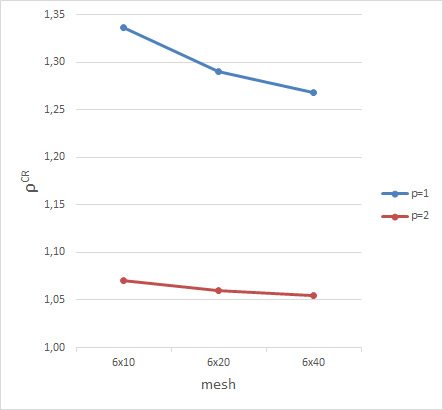
\includegraphics[width=200pt]{ro1.png}
  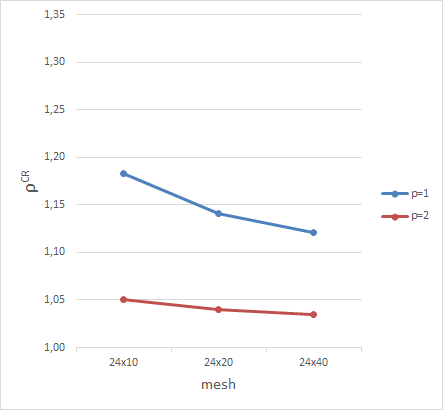
\includegraphics[width=200pt]{ro2.png}
  \caption{$\rho_{CR}$ versus mesh.}
  \label{fig:3}
\end{figure}

Among the codes listed in Table \ref{t-5}, the closest result belongs to the KIKO3DMG code \cite{pataki} with ultrafine grid in plane. Results obtained by earlier versions of the DYN3D, KIKO3D and HEXTRAN codes show a deviation in $\rho_{CR}$ ranging from 4.4\% to 7.4\%. For new and improved version of KIKO3DMG and DYN3D / HEXNEM2 this deviation is rather better. Our results obtained using coarse mesh (6 triangles in plane) and second order of finite elements show good results.

We performed calculations of the AER-2 benchmark transient using relatively coarse meshes and finite elements of first and second orders. As seen in Figure \ref{fig:3}, use of first order finite elements leads to overestimation of the ejected rod worth, especially using coarse meshes. Calculations with second order finite elements give more smooth dependence on mesh type. 

Figure \ref{fig:4} demonstrates some results of the reactor power evolution calculation in comparison with the KIKO3DMG results. We can see that there is convergence of the results for n=6 and p=2. The only calculation was performed using n=24, z=10 and p=2; the obtained results are rather close to the KIKO3DMG results.

We expect that calculations with higher values of (n,z,p) parameters will show more accurate results with evident convergence. This is aim of our future activity.

\begin{figure}[!h]
  \centerline{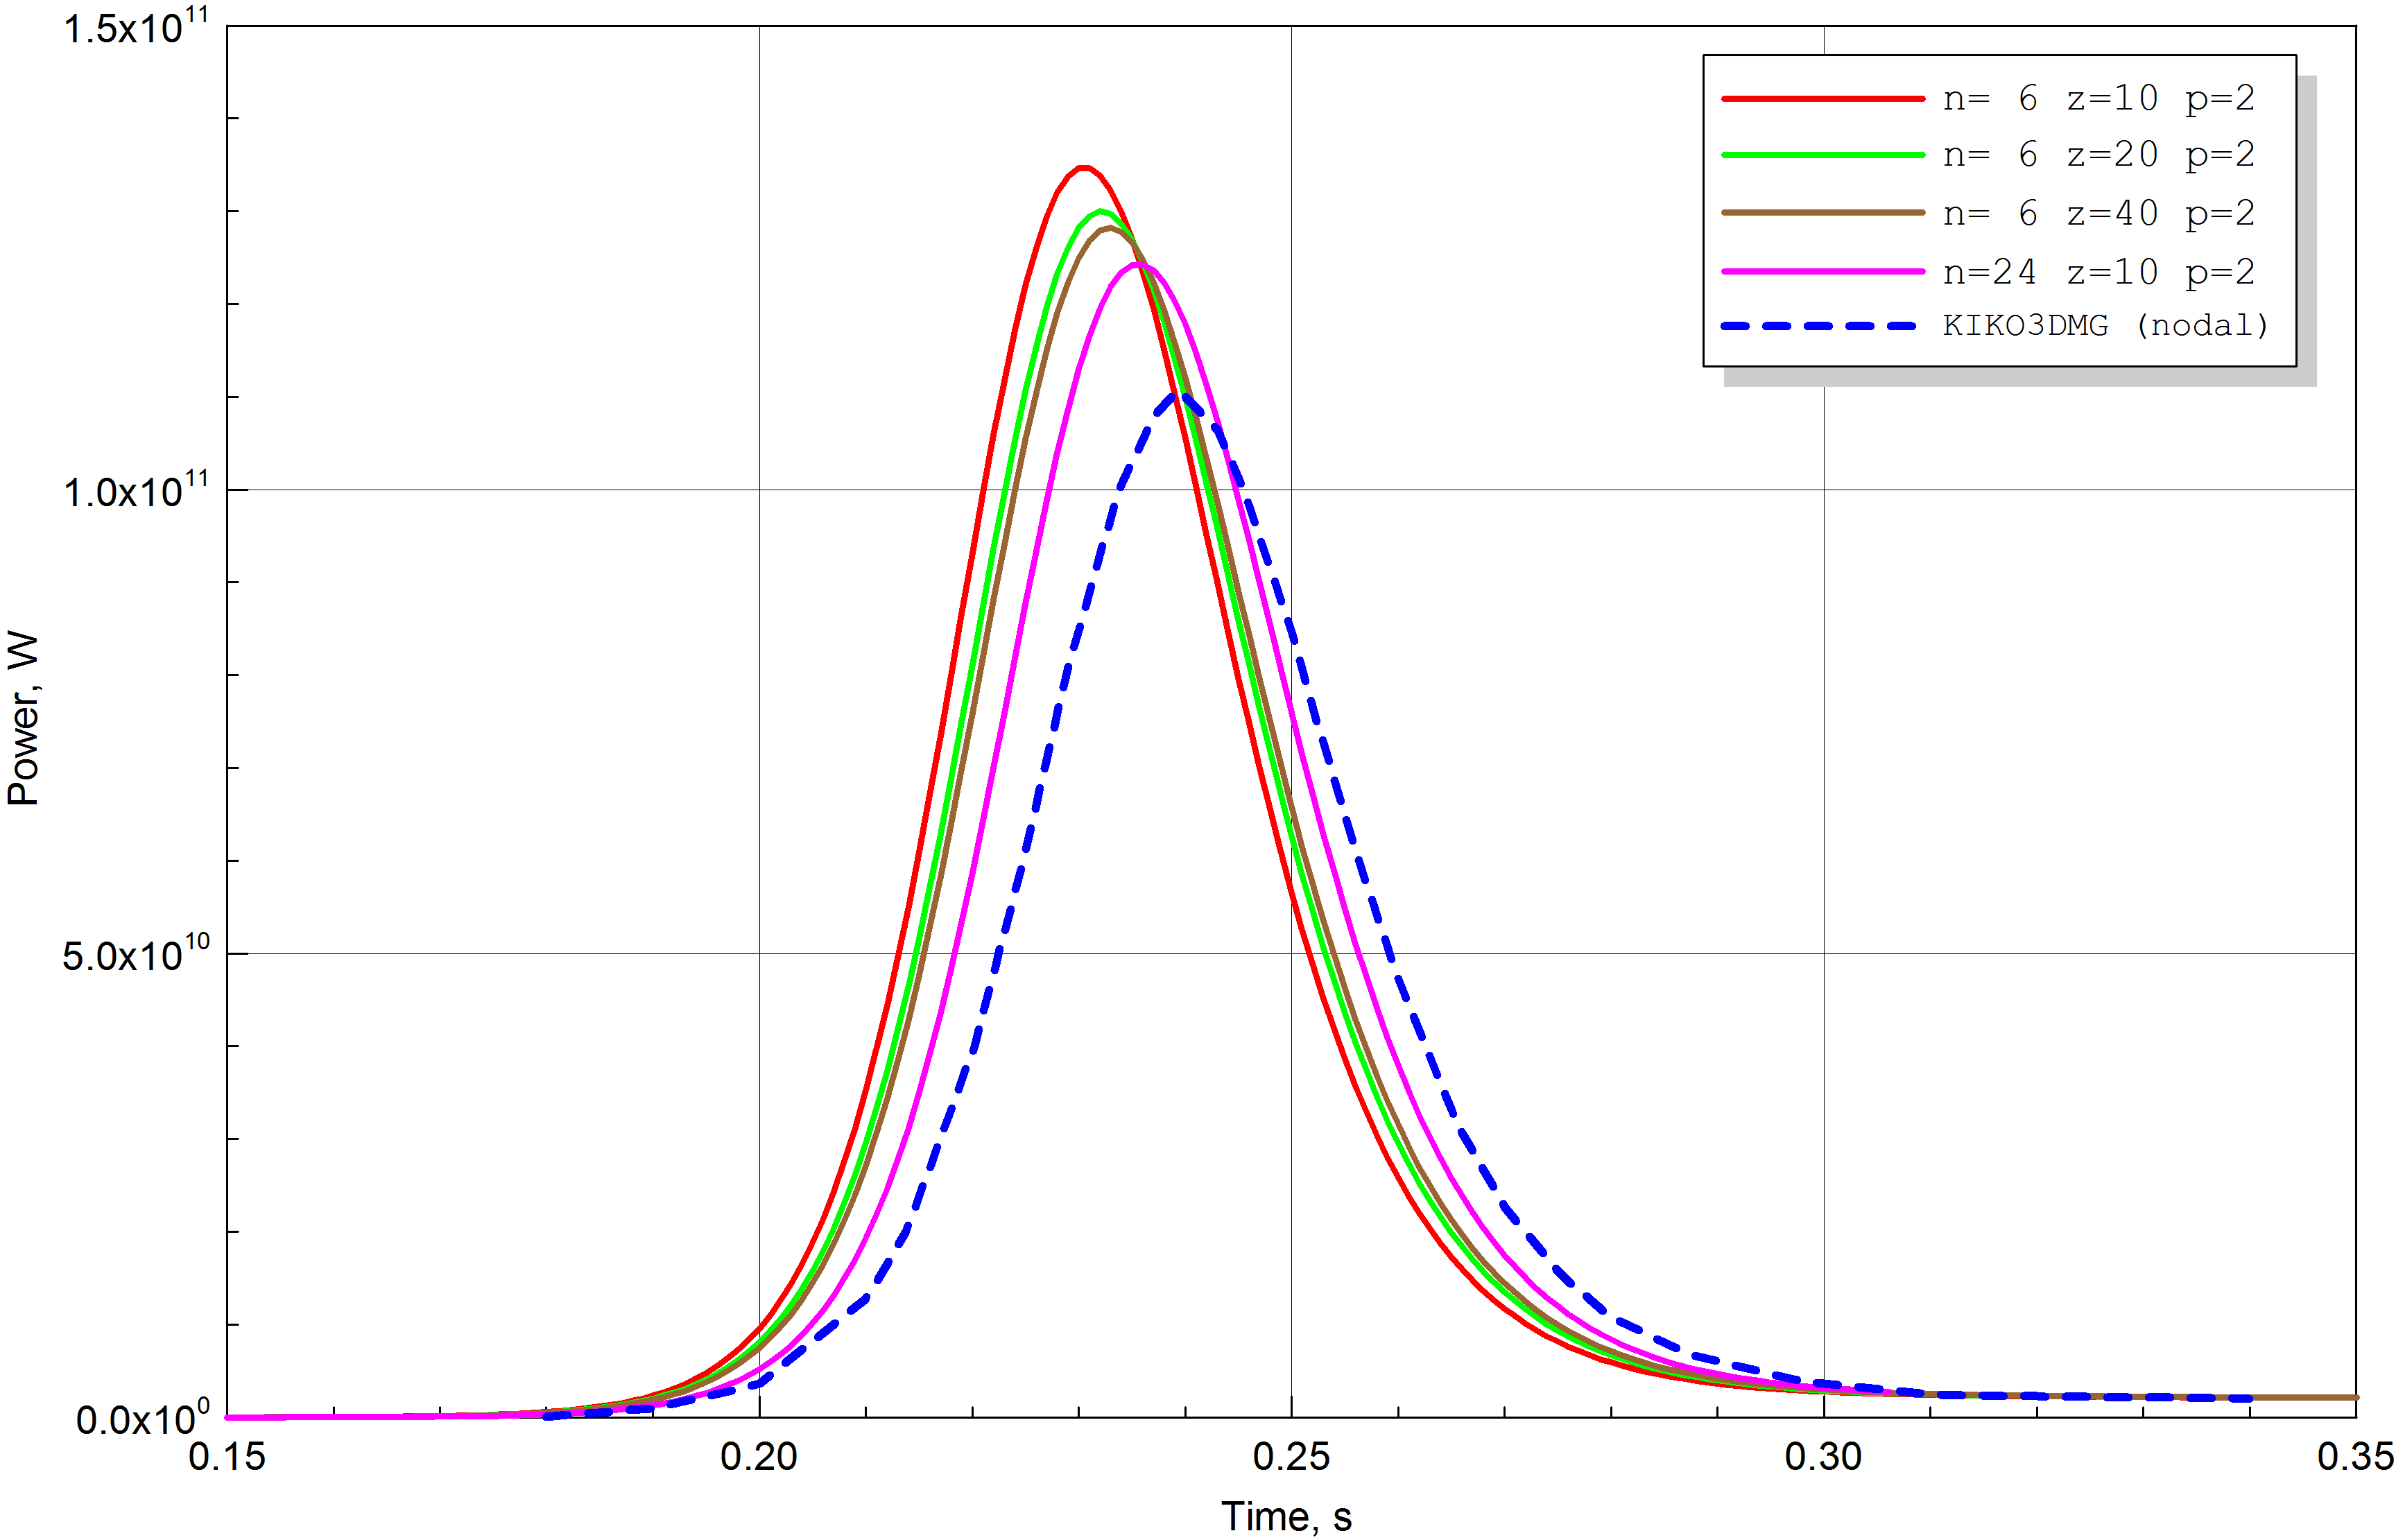
\includegraphics[width=300pt]{power.png}}
  \caption{Power versus time.}
  \label{fig:4}
\end{figure}

\section{ACKNOWLEDGMENTS}
This work was supported by the Russian Foundation for Basic Research (project
16-08-01215 and 15-31-20856) and by the Scientific and Educational Foundation for Young Scientists of Republic of Sakha(Yakutia) 201604010207.

% References

\nocite{*}
\bibliographystyle{aipnum-cp}%

\begin{thebibliography}{35}
\expandafter\ifx\csname natexlab\endcsname\relax\def\natexlab#1{#1}\fi
\expandafter\ifx\csname url\endcsname\relax
  \def\url#1{\texttt{#1}}\fi
\expandafter\ifx\csname urlprefix\endcsname\relax\def\urlprefix{URL }\fi

\bibitem[{Ascher(2008)}]{Ascher2008}
Ascher, U.~M., 2008. Numerical methods for evolutionary differential equations.
  Society for Industrial Mathematics.

\bibitem[{Bell and Glasstone(1970)}]{Bell1970}
Bell, G.~I., Glasstone, S., 1970. Nuclear Reactor Theory. Van Nostrand Reinhold
  Company.

\bibitem[{Brenner and Scott(2008)}]{brenner}
Brenner, S.~C., Scott, R., 2008. The Mathematical Theory of Finite Element
  Methods. Springer.

\bibitem[{Butcher(2008)}]{Butcher2008}
Butcher, J.~C., 2008. {Numerical methods for ordinary differential equations}.
  Wiley.

\bibitem[{Chou et~al.(1990)Chou, Lu, and Chang}]{chou1990three}
Chou, H.~P., Lu, J.~R., Chang, M.~B., 1990. A three-dimensional space-time
  model and its use in pressurized water reactor rod ejection analyses. Nuclear
  Technology 90~(2), 142--154.

\bibitem[{Duderstadt and Hamilton(1976)}]{duderstadt1976nuclear}
Duderstadt, J.~J., Hamilton, L.~J., 1976. Nuclear Reactor Analysis. Wiley.

\bibitem{grossman2007nodal}
Grossman, L.M., Hennart, J.P., 2007. Nodal diffusion methods for space-time neutron
  kinetics. Progress in Nuclear Energy  49(3),  181--216.
  
\bibitem{grundman}
Grundman, U., Rohde, U., 1993. Definition of the second hexagonal kinetic benchmark of AER. Proceedings of the 3rd Symposium of AER. 325/332, KFKI Atomenergia Press.

\bibitem{cronos}
Kolev, N.P., Lenain, R., Fedon-Magnaud, C., 2001. Finite element solutions of the AER-2 rod ejection benchmark by CRONOS. Proceedings of the 11th Symposium of AER, pp. 395/411, KFKI Atomenergia Press.

\bibitem[{Logg et~al.(2012)Logg, Mardal, and Wells}]{fenics}
Logg, A., Mardal, K.~A., Wells, G., 2012. Automated Solution of Differential
  Equations by the Finite Element Method: The FEniCS Book. Springer.

\bibitem[{Marchuk and Lebedev(1986)}]{marchuk1986numerical}
Marchuk, G.~I., Lebedev, V.~I., 1986. Numerical Methods in the Theory of
  Neutron Transport. Harwood Academic Pub.

\bibitem[{Pataki(2013)}]{pataki}
Pataki, I., Keresztúri, A., 2013. Development and verification of new nodal methods in the KIKO3DMG code. Proceedings of the 23nd AER Symposium, Strbske Pleso, Slovakia

\bibitem[{Quarteroni and Valli(2008)}]{quarteroni}
Quarteroni, A., Valli, A., 2008. Numerical Approximation of Partial
  Differential Equations. Springer.

\bibitem[{Stacey(2007)}]{stacey}
Stacey, W.~M., 2007. Nuclear Reactor Physics. Wiley.

\bibitem[{Sutton and Aviles(1996)}]{sutton1996diffusion}
Sutton, T.~M., Aviles, B.~N., 1996. Diffusion theory methods for spatial
  kinetics calculations. Progress in Nuclear Energy 30~(2), 119--182.


\end{thebibliography}


\end{document}
